\chapter*{Задание №2}
Задание: предок ждет завершения своих потомком, используя системный вызов wait(). Вывод соответствующих сообщений на экран. В программе необходимо, чтобы предок выполнял анализ кодов завершения потомков.

\begin{lstlisting}[label = wait, caption=Использование системного вызова wait().]
#include <unistd.h>
#include <stdio.h>
#include <sys/wait.h>

#define FORK_ERROR -1
#define FORK_OK 0

#define COUNT_CHILDS 3

int main(void)
{
	pid_t childs_pid[COUNT_CHILDS];
	pid_t child_pid;
	
	printf("Parent - pid: %d, pgrp: %d\n", getpid(), getpgrp());
	
	for (int i = 0; i < COUNT_CHILDS; i++)
	{
		child_pid = fork();
		if (child_pid == FORK_ERROR)
		{
			perror("Can't fork.\n");
			return 1;
		}
		else if (child_pid == FORK_OK)
		{
			sleep(2);
			printf("Child - pid: %d, ppid: %d, pgrp: %d\n",
			        getpid(), getppid(), getpgrp());
			return 0;
		}
		else{
			childs_pid[i] = child_pid;
		}
		
	}
	
	for (int i = 0; i < COUNT_CHILDS; i++)
	{
		int status;
		pid_t child_pid;
		child_pid = wait(&status);
		
		printf("Child has finished - pid: %d\n", child_pid);
		
		int stat_val;
		if (WIFEXITED(stat_val)){
		   printf("Child exited with code %d\n", WEXITSTATUS(stat_val));
		}
		else {
			printf("Child terminated abnormally.\n");
		}
	}
	
	printf("Parent-child_1_pid: %d, child_2_pid: %d, child_3_pid: %d\n",
	       childs_pid[0], childs_pid[1], childs_pid[2]);
	printf("Parent process is dead\n");
	
	return 0;
}
\end{lstlisting}


Результат работы программы представлен на рисунке \ref{png:res_2}:

\begin{figure}[H]
	\centering{
		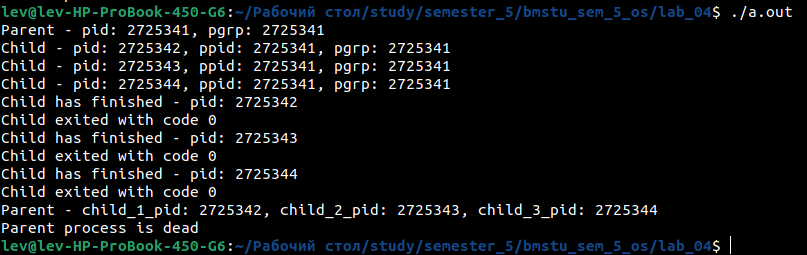
\includegraphics[scale=0.5]{../../../../../../../msys64/home/Лев/bmstu_sem_5_os/lab_04/report/images/task_2}
		\caption{Демонстрация работы программы (задание 2).}
		\label{png:res_2}}
\end{figure}